% !TEX encoding = UTF-8
% !TEX TS-program = pdflatex
% !TEX root = ../tesi.tex

%**************************************************************
\chapter{Lo stage}
\label{cap:descrizione-stage}
%**************************************************************

%**************************************************************
\section{Presentazione del progetto Stargate}

Il progetto dello stage consiste nella realizzazione di una libreria \gls{TypeScript} per applicazioni web, che permetta di aprire qualsiasi componente di User Interface (UI) in una nuova pagina mantenendo lo stato sincronizzato con l'applicazione padre. Tale libreria è denominata \textbf{Stargate}, ispirandosi all'omonima serie televisiva di fantascienza incentrata su portali spaziali nelle diverse galassie. Idealmente la libreria dovrebbe funzionare per qualsiasi applicazione web scritta in \gls{JavaScript}, tuttavia il requisito obbligatorio minimale è che si integri con librerie \gls{React} e \gls{Redux} col minor sforzo possibile.\\

La prima fase dello stage richiede dunque la realizzazione di un Proof of Concept che verifichi in vitreo la possibilità di spostare un componente UI React dalla finestra principale (\textit{padre}) verso una nuova \textit{figlia}, mantendo lo stato consistente. Tali componenti UI sono identificati col nome di \textit{widget}, qualora siano mostrati su una pagina separata.

Un widget deve continuare a visualizzare i dati provenienti dal padre e, se questi si aggiornano, anche il componente nella finestra figlia deve aggiornarsi consistemente. Viceversa le interazioni utente nel componente devono essere propagate alla pagina principale. In sostanza, il componente deve esibire lo stesso comportamento di quando si trovi nell'applicazione principale, sebbene fisicamente si trovi su una diversa pagina del browser.

Infine non vi devono essere vincoli sul numero di componenti aperte in contemporanea su pagine diverse, sia che siano componenti di tipologia diversa sia che siano lo stesso componente istanziato molteplici volte ma indipendenti tra loro.\\

In secondo luogo, è necessario integrare \textit{Stargate} all'interno del prodotto \textit{Route Manager} implementando la possibilità di estrarre la mappa Google Maps su una nuova pagina. L'obiettivo è permettere all'utente di visualizzare le informazioni sulla mappa secondo molteplici prospettive a sua discrezione, ad esempio mostrandolo tutti i veicoli su una pagina, solo una singola rotta real-time su un'altra. Inoltre permette di usufuire della mappa su schermi multipli, funzionalità fortemente desiderata in quanto la mole delle informazioni a schermo è elevata e l'applicazione principale mostra difficoltà nel visualizzarle tutte in una sola pagina web.\\

Lo sviluppo di \textit{Stargate} dovrà dunque avere le seguenti caratteristiche:

\begin{itemize}
    \item Supporto multi-finestra di componenti React;
    \item Supporto per grandi moli di dati, ad esempio geospaziali, in continuo aggiornamento;
    \item Possibilità di eseguire il componente in una nuova pagina che risieda su un processo separato del sistema operativo, affinché alleggerisca il carico computazione dell'applicazione principale. In particolare questa caratteristica è utile per evitare che i calcoli geospaziali vengano eseguiti dal processo padre;
    \item Supporto a molteplici finestre in contemporanea, tutte sincronizzate rispetto all'applicazione padre;
    \item Supporto obbligatorio unicamente per i browser moderni Google Chrome e Firefox. Gli utenti che utilizzino browser non compatibili con \textit{Stargate}, potranno usuguire della normale esperienza utente ma senza la possibilità di aprire nuove finestre;
    \item Supporto a multi-sessione. Qualora l'utente apra due istanze dell'applicazione padre ed in ognuna crei una nuova finestra per un componente, ciascuno di questi deve essere sincronizzato col rispettivo padre e non deve creare conflitti con l'altra applicazione principale.
\end{itemize}

%**************************************************************
\section{Obiettivi}

Si farà riferimento agli obiettivi secondo le seguenti notazioni:

\begin{itemize}
    \item \textbf{O} per i requisiti obbligatori, vincolanti in quanto obiettivo primario richiesto dal committente;
    \item \textbf{D} per i requisiti desiderabili, non vincolanti o strettamente necessari, ma dal riconoscibile valore aggiunto;
    \item \textbf{F} per i requisiti facoltativi, rappresentanti valore aggiunto non strettamente competitivo.
\end{itemize}

Le sigle precedentemente indicate saranno seguite da una coppia sequenziale di numeri, identificativo del requisito. Si quindi prevede lo svolgimento dei seguenti obiettivi:

\begin{table}[!h]
\begin{tabular}{ |p{3cm} |p{9cm}|}
\hline
\textbf{ID} & \textbf{Descrizione} \\ \hline

\multicolumn{2}{|c|}{\textbf{Obbligatori}} \\ \hline

O01 & Supporto multi-finestra di componenti React \\ \hline
O02 & Supporto per grandi moli di dati in continuo aggiornamento, dell'ordine di alcuni MByte \\ \hline
O03 & Supporto a molteplici finestre in contemporanea, tutte sincronizzate rispetto all'applicazione padre \\ \hline
O04 & Supporto per i browser moderni Google Chrome v56 e Firefox v38 \\ \hline
O05 & Supporto a multi-sessione \\ \hline
O06 & Gestione della configurazione di \textit{Route Manager} per supportare i widget \\ \hline
O07 & Produzione della documentazione d'uso di \textit{Stargate} \\ \hline
O08 & Utilizzo del linguaggio TypeScript v3 \\ \hline

\multicolumn{2}{|c|}{\textbf{Desiderabili}} \\ \hline

D01 & Possibilità di eseguire il componente in una nuova pagina che risieda su un processo separato del sistema operativo \\ \hline
D02 & Supporto prestazionale fino ad almeno 5 tabs simultanee \\ \hline
D03 & Supporto componenti JavaScript non React, ad esempio Angular 2 \\ \hline

\multicolumn{2}{|c|}{\textbf{Facoltativi}} \\ \hline

O04 & Supporto per i browser Internet Explorer v11 e Edge v12 \\ \hline

\end{tabular}
\caption{Tabella degli obiettivi}
\end{table}

%**************************************************************
\section{Pianificazione}

In accordo col tutor Matteo Ronchi, l'attività dello stage è stata suddivisa nelle seguenti fasi:

\begin{itemize}
    \item \textbf{Fase 1}: Analisi dello stato dell'arte per la comunicazione cross-page in JavaScript
    \item \textbf{Fase 2}: Realizzazione Proof of Concept in React e Redux
    \item \textbf{Fase 3}: Progettazione per integrazione in \textit{Route Manager} del widget Google Map. Implementazione dell'integrazione ed evoluzione della libreria.
    \item \textbf{Fase 4}: Validazione e stesura documentazione
\end{itemize}

Non vi è stata necessità di un periodo iniziale di formazione sulle tecnologie TypeScript, React e Redux io quanto già in mio possesso. Mi sono anche trovato subito a mio agio con i processi di sviluppo aziendali, già incontrati da me in altre occasioni.

Essendo inoltre un'attività di Ricerca e Sviluppo, vi è stata una continua interazione col tutor aziendale per la definizione dei successivi step, ma a monte è stata pianificata un'ipotetica suddivisione delle ore nel seguente modo: \\

\begin{table}[!h]
\begin{tabular}{ |p{2cm} |p{10cm}|}
\hline
\textbf{Ore} & \textbf{Descrizione dell'attività} \\ \hline

40 & Analisi dello stato dell'arte tecnologico \\ \hline
80 & Realizzazione Proof of Concept in React e Redux \\ \hline
32 & Progettazione architteturale \\ \hline
104 & Integrazione in \textit{Route Manager} del widget Google Map \\ \hline
24 & Gestione configurazione per supportare widget \\ \hline
16 & Validazione e Collaudo \\ \hline
8 & Refactoring prima del rilascio in produzione \\ \hline
8 & Stesura documentazione \\ \hline

\multicolumn{2}{|c|}{\textbf{Totale: 312 ore}} \\ \hline

\end{tabular}
\caption{Tabella della suddivisione delle ore}
\end{table}

\begin{figure}[!h] 
    \centering 
    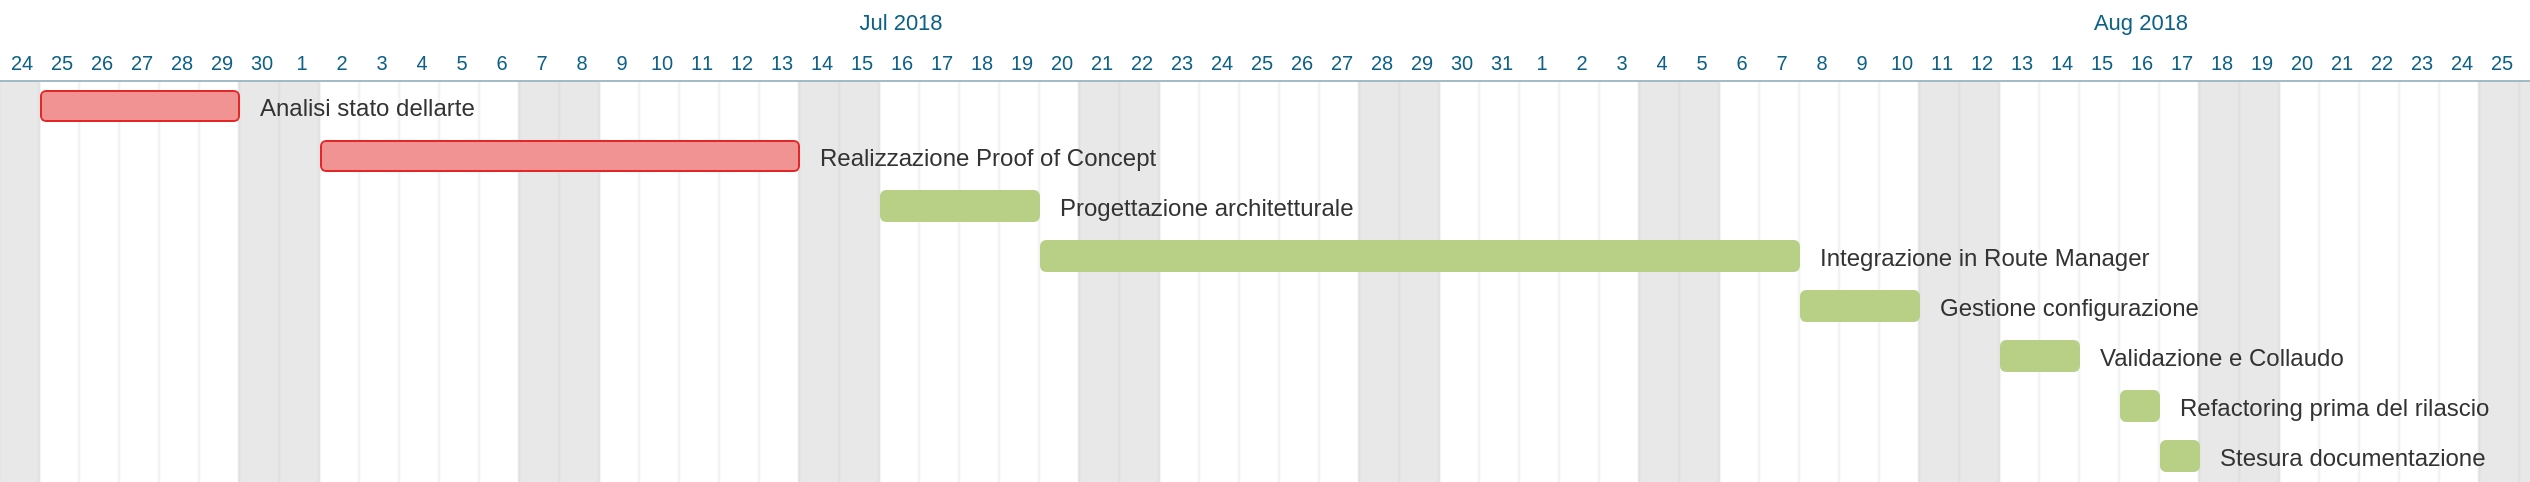
\includegraphics[width=0.9\columnwidth]{gantt} 
    \caption{Diagramma Gantt della pianificazione}
\end{figure}

%**************************************************************
\section{Analisi preventiva dei rischi}

Durante la fase di analisi iniziale sono stati individuati alcuni possibili rischi a cui si potrà andare incontro.
Si è quindi proceduto a elaborare delle possibili soluzioni per far fronte a tali rischi.\\

\begin{table}[!h]
\begin{tabular}{ |p{6cm} |p{6cm} |p{3cm}|}
\hline
\textbf{Descrizione} & \textbf{Piano di emergenza} & \textbf{Rischio} \\ \hline
Difficoltà tecnologica: vi è il rischio che lo stato dell'arte dello sviluppo web non consenta di aprire finestra come processi separati o che non sia possibile effettuare la comunicazione tra pagine diverse. & È importante effettuare un'attenta attività di ricerca iniziale, al fine di comprendere lo stato dell'arte per quanto riguarda la comunicazione cross-page in applicazioni web. \newline In caso di difficoltà nella ricerca della soluzione tecnica ideale, si adotterà quella con miglior compromesso di affidabilità-performance tra quelle disponibili. & Occorrenza: Alta \newline Pericolosità: Alta \\ \hline

Difficoltà di integrazione: vi è il rischio che non sia possibile integrare le tecnologie adottate nel contesto dell'applicazione \textit{Route Manager}, in quanto è già in sviluppo da oltre un anno e non progettata in partenza per essere multi-finestra. & In caso di verifica del rischio, si analizzerà il problema col tutor interno Matteo Ronchi per trovare la miglior soluzione da adottare in \textit{Stargate} oppure in \textit{Route Manager} & Occorrenza: Alta \newline Pericolosità: Alta \\ \hline
\end{tabular}
\caption{Tabella dell'analisi dei rischi}
\end{table}
